%\begin{document}
\chapter{水声信道特点与自适应均衡技术}
%==========================================================================
\thispagestyle{empty}
%==========================================================================
\section{水声信道的特点}
根据通信系统的使用环境,通信信道可分为:无限带宽信道,限带信道和多径衰落信道\citep{ProakisB2001}。这三类信道均受到噪声的干扰。无限带宽信道具有固定的信道衰减和相移,限带信道具有确定的或随时间缓慢变化的信道冲激响应,多径衰落信道具有随机时变冲激响应特性。水声信道的传播速度低,可用带宽窄、时变、多径衰落信道。温度、盐度、深度、风、浪、流以及航运、海底工程等人类活动都对水声信道产生直接而显著的影响,与无线电波信道相比,水声信道要恶劣得多。深刻了解水声信道的传播特点,以及这些特点对水声信号产生了什么影响,是研究水下声通信技术的主要切入点之一。
%***************************************************************************
\subsection{水声信道模型}
对于水声信道这样的物理信道,会导致发送信号的时变、多径传播,在数学上我们可以将其表征为时变线性滤波器。该滤波器可以表征为时变信道冲激响应$c(\tau,t)$,它是信道在$t-\tau$时刻加入冲激而在$t$时刻的响应。对于输入信号$s(t)$,信道输出为:
\begin{eqnarray}
    \begin{array}{l@{\;=\;}l}
        r(t)&s(t)*c(\tau,t)+n(t)\\
        &\displaystyle\int_{-\infty}^{\infty}c(\tau,t)s(t-\tau)d\tau+n(t)\\
    \end{array}
    \label{equ:2.1}
\end{eqnarray}
用来表征通过物理信道的多径信道传播的模型是式(\ref{equ:2.1})的一个特例,该特例中的时变冲激响应为:
\begin{eqnarray}
    c(\tau,t)=\sum_{k=1}^La_k(t)\delta(\tau-\tau_k)
    \label{equ:2.2}
\end{eqnarray}
式中,$a_k$表示$L$条多径传播路径上可能的时变衰落因子,$\tau_k$表示相应地时间延迟。

将式(\ref{equ:2.2})代入式(\ref{equ:2.1})中,则接收信号可以表示为:
\begin{eqnarray}
    r(t)=\sum_{k=1}^La_k(t)s(t-\tau_k)+n(t)
    \label{equ:2.3}
\end{eqnarray}
因此,接收信号由$L$个路径分量组成,其中每一个分量的衰减因子为$a_k$,延迟为$\tau_k$。

水声信道是一种典型的时延-多普勒双扩散信道,因此,简单地将水声信道表示成抽头延迟线模型是不合适的。在第四章介绍信道估计算法时将给出水声信道的双扩散模型。
%***************************************************************************
\subsection{双扩散特征}
%---------------------------------------------------------------------------
\subsubsection*{多径效应}
在水声通信系统中,水声信道的多径效应被认为是水声通信中遇到的最大困难。由于海水介质的非均匀性、声传播信道中的海底海面反射、海洋中的各种各样的反射体和散射体的存在以及声波在水声较慢的传播速度,水声信道必然存在多径现象,也就是说在一定波束宽度内发出的声波可沿几种不同的路径到达接收点。由于声波在不同路径中传播时路径长度的差异,到达接收点的声波能量和时间也不相同,从而引起信号的衰落及波形的畸变。

多径效应的形成于海洋环境和信号频率有关,其形成主要机理是声线弯曲和海底、海面的反射,海曙中内部结构如内波、紊流、潮汐等的影响,以及声源和接收机平台的运动等。当声波在不同的层、海底和海面间传播会造成多次的反射和折射,从而形成各个不同的传播路径。水下声信道在相干时间长度内,可简化为相干多径信道,仅仅存在多径效应。

多径传播时影响水声通信系统性能的重要因素之一。多径传播引起信号的时延扩展。在频域上表现为信号的频率选择性衰落。时延扩展又被称为多径扩展,会引起信号的码间干扰。由于海水中内部结构(如内波、水团、湍流等)的影响,多径结构通常是时变的,多径的时变性引起传输信号的频率扩散,导致传输信号产生时间选择性衰落,实际中这两种衰落经常伴随在一起的。

在数字通信系统中,多径传播会造成码间干扰。在无线电信道中,码间干扰通常为几个码元宽度,而在水平传播的水声信道中,对中、高数据率的浅海信道码间干扰将由几十和几百个码元宽度。多径传播造成的码间干扰是影响水声信道系数据率的主要因素。目前,人们常用均衡等技术来对抗多径引起的码间干扰。
%---------------------------------------------------------------------------
\subsubsection*{多普勒频移}
由于发射机和接收机之间的相对运动以及海水流动和湍流的作用,声波在浅海信道传播过程中会产生一定的频率漂移,即为多普勒频移。当收、发机之间有相对运动的情况时,假定发射端和接收端的运动速度分别为$\nu_s$和$\nu_r$,信号的发送频率为$f_s$,则当信号到达接收端时,接收信号的频率$f_r$可以表示为:
\begin{eqnarray}
    f_r=f_s\frac{c-\nu_r}{c-\nu_s}
    \label{equ:2.4}
\end{eqnarray}
上式中,$\nu_s$和$\nu_r$分别是发射机和接收机的速度,单位为米/秒($m/s$),$c$为海水中的声速,一般理论值为$1500m/s$,$f_s$和$f_r$的单位是赫兹(Hz)。

在发射机和接收机没有相对运动的情况下,接收信号的多普勒频移主要受到两个方面的影响:海平面上的波浪影响和海洋内部的湍流作用。我们对这种情况进行了简化:将海绵视为动态的正弦曲线,由于海面波浪的前向散射作用,声信号在传播过程中被调制,在到达接收端时发生了频率偏移,根据Carson定理,我们可以计算出此时接收信号的多普勒频移:
\begin{eqnarray}
    f_d=2f_d\left(1+\frac{2b\cos\theta}{c}h_b\right)
    \label{equ:2.5}
\end{eqnarray}
其中,$f_b$为海面波浪运动的频率,$h_b$为波浪高度的均方根值,$b$为海上风速,单位为$m/s$,$c$为海水中的声速,一般可认为是$1500m/s$,$\theta$为声波到达接收端的入射角。

多普勒扩展时一种由多普勒频移引起的声信号的衰落,即时间选择性衰落。假设有一单频正弦信号的频率为$f_c$,其频谱特性表现为频率$f_c$处的一条频谱轨迹,当这个单频信号被发射后,由于水深信道的多普勒效应对单频信号的影响,致使接收信号的频谱发生了展宽,即从频率为$f_c$的谱线扩展到从$f_c-f_D$至$f_c+f_D$的有限带宽范围内。
%***************************************************************************
\subsection{有限带宽}
水声信道带宽主要由海洋中水声信号的传播损耗所决定,同时还受到水声换能器带宽限制的影响。海洋介质的弛豫吸收\citep{Essebbar1994},界面对声信号的反射、散射以及波阵面几何扩展等因素都造成了水声信号在传输过程中的衰减,严重影响了接收机的工作效率。其中海洋介质对声信号的吸收与水声信号的工作频率有关,频率越高的信号,能量损失的就越多。其平均传播损失为:
\begin{eqnarray}
    TL=20\lg r+\alpha r\times10^{-3}
    \label{equ:2.6}
\end{eqnarray}
上式中传播距离$r$的单位为米,$\alpha$为吸收系数(dB/m),与深度、温度特别是声波频率密切相关。它随着频率的增加而增加,从而大大增加了传播损失。水下数字通信中一般的工作载波频率在$10\textasciitilde
1500\mbox{kHz}$以内,带宽为$200\textasciitilde
4300\mbox{Hz}$,而声波频率在$4000Hz$左右为远距离传输的最佳频率。其中低于$15\mbox{kHz}$为低频带,$15\mbox{kHz}\textasciitilde
150\mbox{kHz}$范围内位中频带,$150\mbox{kHz}\textasciitilde
1500\mbox{kHz}$范围内为高频带。传输距离为$1\textasciitilde10\mbox{km}$的浅海水通信系统工作频率主要在$10\textasciitilde
100\mbox{kHz}$频率范围内;而远距离通信中的工作频段主要在$0\textasciitilde
20\mbox{kHz}$。由此可见,低频段的声波将在远距离水声通信中有着广泛的应用。
%***************************************************************************
\subsection{声波传播损失}
由于海水中以硫酸镁和硼酸镁为主要成分的不均匀介质对信号的弛豫吸收作用、海洋环境的多变性以及声传播过程中的波阵面几何扩散,使得声音信号在传播过程汇总损耗严重,严重影响了接收机的接收效率。

传输损耗是指声波在海水中传播时,由于扩散和衰减引起声波发生延迟、失真和衰落。传输损耗有两种:衰减损失和扩散损失。

声波的衰减损失包括吸收、散射和声能漏出声道的效应。当声波频率在$1\mbox{kHz}$以上时,海水对声波的吸收是造成声波衰减的主要因素,与声波频率的平方成正比,Thorp等人在综合了大量的测量结果之后,给出了海水(含盐度$3.5\%$,$\mbox{MgSO}_4$在海水溶解盐中比重为$4.7\%$)对声波的吸收系数经验公式:
\begin{eqnarray}
    \alpha=\frac{0.11f^2}{1+f^2}+\frac{44f^2}{4100+f^2}
    \label{equ:2.7}
\end{eqnarray}
其中,$f$为以千赫兹计的频率,$\alpha$单位:分贝/公里。从式(\ref{equ:2.7})可以看出,海水中的声吸收系数主要取决于工作频率。
\begin{figure}[htb]
  \begin{center}
    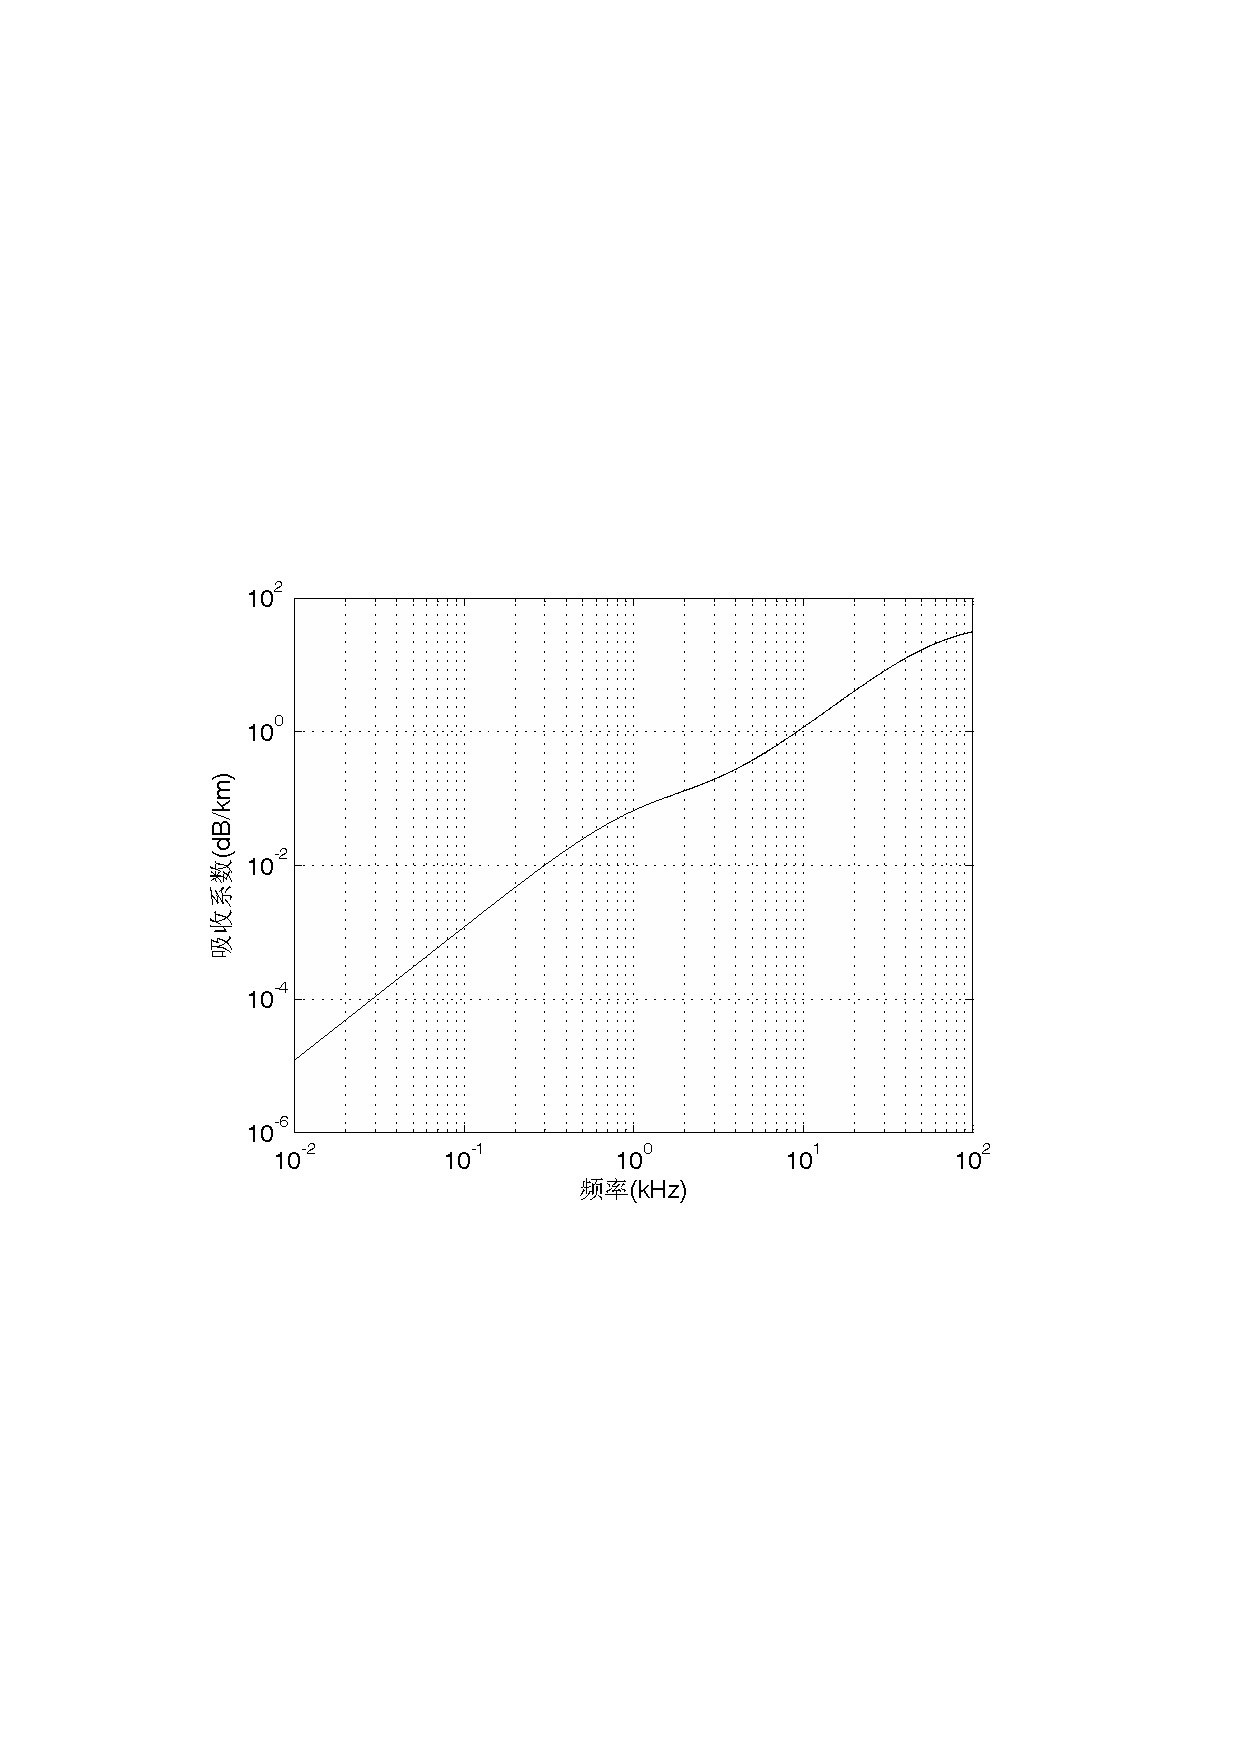
\includegraphics[width=0.8\textwidth]{images/alphacoe.pdf}
  \end{center}
  \caption{海水对声波的低频吸收系数}
  \label{fig:2.1}
\end{figure}
从曲线变化可以看出:随着工作频率的增加,吸收系数是单调上升的。所以海水对声波的吸收衰落是限制水声通信工作频率的主要因素。对于中远距离来说,一般的工作载波频率在$20\mbox{kHz}$以下。

声波的扩散损失是表示当声信号从声源向外扩展时有规则减弱的几何效应。在中远距离上,随距离$R$的增加,声能量按$\frac{1}{R^{\frac{3}{2}}}$衰减,这就是著名的反二分之三次方衰减规律。水声信道对声波的扩散损失决定了水声通信设备的最大作用距离。
%***************************************************************************
\subsection{环境噪声}
在海洋中有许多噪声源,包括潮汐、湍流、海面波浪、风成噪声、生物噪声、航船以及工业噪声等,噪声的性质与噪声源有密切的关系,在不同的时间、深度和频段有不同的噪声源。在水声学中,通常用环境噪声级来描述环境噪声。

水声信道的噪声是非高斯分布的。不同的声源有着不同的带宽和噪声级,且随时间和空间变化。因此,要给出噪声的统计表达式是很困难的。实验观察可以发现,在$10\mbox{Hz}$以下的噪声主要来源于海洋的扰动,频率在$10\mbox{Hz}$到$500\mbox{Hz}$之间的噪声主要来源于航船和地理位置,对于较高频率噪声,即频率在$500\mbox{Hz}$到$50\mbox{kHz}$的噪声,主要来源于海面的不平整,而对于超过$50\mbox{kHz}$的噪声,则主要来源于海水中的分子移动。

在浅海信道,生物活动和沿岸工业也是信道噪声的来源。而且,噪声随着时间、日期、季节、地理位置、航船密度和天气的变化将产生一个很大的变化范围。所有的这些,将使浅海信道成为一个严重的时变、空变噪声信道。
%==========================================================================
\section{自适应均衡技术}
%***************************************************************************
\subsection{自适应均衡技术综述}
信道均衡是通信技术和信号处理的基本问题之一,其目的在于克服传送符号间的码间干扰,这种干扰是因为信道的非理想特性造成的,由于水声信道的特性具有时变性,因此需要自适应的调整均衡器,使得整个传输系统传输的符号间干扰被消除,这种均衡器被称为自适应均衡器。

自适应均衡过程一般包括训练和跟踪两种模式。首先,由发射机发射一系列已知的固定长度的训练序列,均衡器抽头根据训练序列作一定的调整。通常的训练序列是一串预先指定的数据或一组伪随机信号,发射机在发送训练序列后发送用户数据,经过训练的均衡器在判决引导模式完成对抽头系数的调整,对信道做出跟踪补偿。

训练序列的设计必须能够在最恶劣的信道条件下,当训练序列结束以后,能使得均衡器系数接近最优。这样,当接收用户数据时,自适应均衡器就能够跟踪信道的变化。为了保证始终有效的ISI,需要周期的重复不断的训练均衡器。因为在数字通信中用户数据是被分为若干段放在相应地时间段中传送的,所以均衡器被大量用于数字通信中。

第一个自适应滤波器(或者自学习滤波器)通常归功于Lucky,他曾在1966年为了补偿数据传输系统产生的畸变而设计了一种迫零均衡器。然而,早在1960年,Jakowatz等人在自适应波形识别研究中已经报告了类似的工作。有关自适应滤波器方面的理论研究由Giaser和英国的Gabor等人在1961年报道,他们将它用于模拟磁带传输机构中以调整非线性“学习滤波器”的权系数。

自适应滤波器的这些早期成果许多是在各个研究机构独立的取得的。除了上面提到的,另外一些有价值的早期工作是由德国的卡尔斯卢埃技术学院和斯坦福大学完成的,他们从1959年起就开始研究自适应模型识别系统。1964年,这两个单位之间的合作交流使得双方都有机会评论对方的技术,取长补短,这样就促进了用途最广泛的调整处理器权系数的算法和研究。其相关的研究同时也在莫斯科的自动化和遥控机械研究所内展开。在60年代中,Rudian发表了有关自适应滤波器进展现状的书面综述及其在自动均衡应用方面的早期参考资料。更晚些时候,Weinstein在电话回波抵消,Qureshi在自适应均衡方面发表了简要评述。

有许多方法可以用来调整滤波器的权系数值,以获得最优解,下面就对自适应均衡算法作简单介绍。
%***************************************************************************
\subsection{自适应均衡算法}
自适应均衡器要采用自适应信号处理算法来调整可调参数滤波器的系数。广泛采用的算法主要有两大类\citep{Simon2001},即最小均方(LMS)类算法和递归最小二乘(RLS)类算法。LMS算法以其计算复杂度低,结构简单而得到广泛应用。但它的收敛速度慢,针对这个问题又研究出许多自适应LMS类算法,如归一化LMS算法、变换域LMS算法、快随自优化LMS算法等。RLS类算法有运算复杂度、计算量大的缺点,但其收敛性能较好。尽管自适应算法类型很多,但最终都源于LMS和RLS这两类算法。

\subsubsection*{LMS算法}
\begin{figure}[htb]
  \begin{center}
    \includegraphics[width=0.8\textwidth]{images/linearFilter.pdf}
  \end{center}
  \caption{基本LMS算法框图}
  \label{fig:2.2}
\end{figure}
最小均方算法是基于最小均方误差准则的自适应算法。其基本思想是通过调整滤波器系数使均方误差最小。它由最陡下降算法推导出来。最陡下降算法是基于统计的观点(集平均),通过递推法得到最优权值,但是它的主要限制是需要准确测得每次迭代的梯度矢量的方法\citep{Simon2001},故只在统计平均的意义下才与最陡下降梯度下降法等效,其解与后者相比也呈现不同程度的波动。尽管如此,LMS算法仍以其简洁的原理和算法受到重视,在自适应领域中占有非常重要的地位。

设输入信号为$\mathbf{Z}_{\mathrm{N}}(n)=[z(n),z(n-1),\cdots,z(n-N+1)]^{\mathrm{T}}$,延迟抽头(权系数)为$\mathbf{W}_{\mathrm{N}}(n)=[w_0(n),w_1(n),\cdots,w_{N-1}(n)]^{\mathrm{T}}$,信号的真实值为$x(n)$,输出$\hat{x}(n)$是输入的加权值,则:
\begin{eqnarray}
    \hat{x}(n)=\mathbf{W}_{\mathrm{N}}^{\mathrm{H}}(n)\mathbf{Z}_{\mathrm{N}}(n)
    \label{equ:2.8}
\end{eqnarray}
\begin{eqnarray}
    e(n)=x(n)-\hat{n}(n)
    \label{equ:2.9}
\end{eqnarray}
\begin{eqnarray}
    J(n)=\mathrm{E}(|e(n)|^2)
    \label{equ:2.10}
\end{eqnarray}
\begin{eqnarray}
    \mathbf{W}_{\mathrm{N}}(n+1)=\mathbf{W}_{\mathrm{N}}(n)-\mu\nabla(J(n))
    \label{equ:2.11}
\end{eqnarray}
其中,上标$H$表示共轭转置。

由式(\ref{equ:2.11})可见,要得到LMS算法的更新公式,须确定$\nabla(J(n))$及合适选择步长因子$\mu$。

我们可以按照下面的方法得到$\nabla(J(n))$的估计值:
\begin{eqnarray}
    \nabla(J(n))=\nabla(|e(k)|^2)=-2e^*(n)\mathbf{Z}_{\mathrm{N}}(n)
    \label{equ:2.12}
\end{eqnarray}
可以证明梯度的估计值是无偏估计,即:
\begin{eqnarray}
    \mathrm{E}(\nabla(J(n)))=\nabla(J(n))
    \label{equ:2.13}
\end{eqnarray}
将式(\ref{equ:2.12})代入式(\ref{equ:2.11})得:
\begin{eqnarray}
    \mathbf{W}_{\mathrm{N}}(n+1)=\mathbf{W}_{\mathrm{N}}(n)-\mu\mathbf{Z}_{\mathrm{N}}(n)e^*(n)
    \label{equ:2.14}
\end{eqnarray}
式(\ref{equ:2.8})、(\ref{equ:2.9})和(\ref{equ:2.14})共同构成了LMS算法。
对于$\mu$的选择,须满足:
\begin{eqnarray}
    0<\mu<\frac{2}{\lambda_{\mathrm{max}}}
    \label{equ:2.15}
\end{eqnarray}
$\lambda_{\mathrm{max}}$是输入信号自相关矩阵$R_x$的最大特征值。步长因子$\mu$对算法收敛过程有很大的影响,过大或过小都是不合适的。

当信道特征稳定时,存在一个最优的$\mu$值使$\mathbf{W}_{\mathrm{N}}(n)$经过有限次迭代后达到最优。但是,对于起伏较大的信道,固定$\mu$值的LMS算法就不能取得好的结果。若$\mu$值能够随信道特性自适应变化,便可改善LMS算法的信道跟踪性能,于是便有了快速自优化LMS(FOLMS)算法。
\subsubsection*{快速自优化LMS算法(FOLMS)}
LMS算法仅有一个控制因子$\mu$,LMS算法的特性主要取决于$\mu$值的选取,为了保证算法收敛,通常需要把$\mu$取得较小,但是有时要求快速收敛,又需要将$\mu$值取的尽量大一点。因此实际应用汇总$\mu$的选取往往很困难,其取值直接影响了算法的收敛及跟踪速度和稳定性。

考虑到在每步更新过程中,肯定存在一个最优的$\mu$,使权系数$\mathbf{W}_{\mathrm{N}}(n)$在更新时能达到瞬时最优,如果$\mu$已经固定,LMS算法就不可能有非常好的效果。此时应当考虑使$\mu$能够随系统的变化而自适应地变化的方法,快速自优化LMS算法(Fast
Self-Optimized
LMS),简称FOLMS算法,就是一种快速的自优化LMS算法\citep{Bragard1990,George1999,Benveniste1990}。

正如前面所说,对于LMS算法来说,算法每次更新自适应滤波器权系数$\mathbf{W}_{\mathrm{N}}(n)$时一定存在一个最优的$\mu$,使得MSE最小。因此,推导FOLMS算法的基本思想是通过MSE对$\mu$求导数,写出$\mu$的递推更新公式,使之随着MSE的变化自适应调节,逐步地最小化均方误差。这样就可以肯定取得比LMS算法更好的跟踪时变的能力。

由前面可知MSE的代价函数为:
\begin{eqnarray}
    J(n)=\mathrm{E(|e(n)|^2)}
    \label{equ:2.16}
\end{eqnarray}
式中:
\begin{eqnarray}
    e(n)=x(n)-\mathbf{W}_{\mathrm{N}}(n)^{\mathrm{H}}\mathbf{Z}(n)
    \label{equ:2.17}
\end{eqnarray}
将式(\ref{equ:2.16})对$\mu$求导,得到$J(n)$对$\mu$的梯度$\nabla_{\mu}(n)$:
\begin{eqnarray}
    \nabla_{\mu}(n)=\frac{\partial J(n)}{\partial
    \mu}=\mathrm{E}\left(\frac{\partial e(n)}{\partial
    \mu}e^*(n)+\frac{\partial e^*(n)}{\partial \mu}e(n)\right)
    \label{equ:2.18}
\end{eqnarray}
由式(\ref{equ:2.17})可得:
\begin{eqnarray}
    \frac{\partial e(n)}{\partial \mu}=-\boldsymbol{\Psi}^{\mathrm{H}}\mathbf{Z}(n)
    \label{equ:2.19}
\end{eqnarray}
上式中,$\boldsymbol{\Psi}(n)$表示权向量$\mathbf{W}_{\mathrm{N}}(n)$对$\mu$的梯度:
\begin{eqnarray}
    \boldsymbol{\Psi}(n)=\frac{\partial\mathbf{W}(n)}{\partial\mu}
    \label{equ:2.20}
\end{eqnarray}
因此式(\ref{equ:2.18})可以改写为:
\begin{eqnarray}
    \begin{array}{l@{\;=\;}l}
        \nabla_{\mu}(n)&-\mathrm{E}(\boldsymbol{\Psi}^{\mathrm{H}}(n)\mathbf{Z}(n)e^*(n)+\mathbf{Z}^{\mathrm{H}}(n)\boldsymbol{\Psi}(n)e(n))\\
        &2\mathrm{Re}[\boldsymbol{\Psi}^{\mathrm{H}}(n)\mathbf{Z}(n)e^*(n)]
    \end{array}
    \label{equ:2.21}
\end{eqnarray}
其中的$\mathrm{Re}[\cdot]$表示对复数取实部。

借助于LMS算法中用瞬时梯度代替平均梯度的思想,我们也可以得出$\mu$值的更新递推算法:
\begin{eqnarray}
    \mu(n+1)=\mu(n)-\alpha\nabla_{\mu}(n)
    \label{equ:2.22}
\end{eqnarray}
其中的$\alpha$是一个很小的常数。

整个FOLMS算法可以归纳如下:
\begin{eqnarray}
    \begin{array}{r@{\;=\;}l}
        \hat{x}(n)&\mathbf{W}_{\mathrm{N}}(n)^{\mathrm{H}}\mathbf{Z}(n)\\
        e(n)&x(n)-\hat{x}(n)\\
        \mathbf{W}_{\mathrm{N}}(n+1)&\mathbf{W}_{\mathrm{N}}(n)+\mu(n)\mathbf{Z}(n)e^*(n)\\
        \mu(n+1)&[\mu(n)-\alpha\mathrm{Re}[\boldsymbol{\Psi}^{\mathrm{H}}(n)\mathbf{Z}(n)e^*(n)]]_{\mu_{\mathrm{min}}}^{\mu_{\mathrm{max}}}\\
        \boldsymbol{\Psi}(n+1)&[\mathbf{I}-\mu(n)\mathbf{Z}(n)\mathbf{Z}^{\mathrm{H}}(n)]\boldsymbol{\Psi}(n)+\mathbf{Z}(n)e^*(n)
    \end{array}
    \label{equ:2.23}
\end{eqnarray}
从上式可以看出,FOLMS算法和LMS算法类似,只是多了更新$\mu$这个环节,该算法在每次更新时大约需要$4N$次的乘法运算,其中$N$为滤波器的阶数。

需要特别指出的是,为了保证算法的稳定性,在实际应用中,更新$\mu$的步骤中需要对其设定门限值$\mu_{\mathrm{max}}$和$\mu_{\mathrm{min}}$。$\mu_{\mathrm{min}}$取一接近于零的正值即可,而$\mu_{\mathrm{max}}$的选取对算法的性能至关重要,需要仔细选取\citep{Geller1996}。
\subsubsection*{RLS算法}
LMS算法尽管简单易懂,但由于其中只有一个可调量$\mu$,性能在一定程度上受到限制,收敛速度慢,收敛所需码元数较多,用以各时刻的抽头参量(即权值)等作该时刻数据块估计时平方误差为最小的准则,而未用现时刻的抽头参量来对以往各时刻的数据块作重新估计后的累计平均误差为最小的准则,故对非平稳信号的适应性差,只有在稳态时才能达到最优解。为了克服上述缺点,我们采用新的准则:在每一时刻对所有已输入信号进行重估的平方误差和最小的准则,即最小二乘准则。这一准则在现有的约束条件下,利用了最多可利用的信息,是更为有效的,对信号的非平稳性适应能力也较LMS准则好。下面,我们还是先简单地推导其算法,推导过程中与前面意义相同或相似的量不再重复加以说明。

递归最小二乘(Recursive Least Square,
RLS)法所遵循的准则是确定$\mathbf{W}_{\mathrm{N}}$,使$e(i|n)=x(i)-{\mathbf{Z}}'_{\mathrm{N}}(i)\mathbf{W}_{\mathrm{N}}(n)$的加权平方和为最小。
\begin{eqnarray}
    \varepsilon(n)=\sum_{i=1}^N\lambda^{n-i}e^2(i|n)
    \label{equ:2.24}
\end{eqnarray}
其中,$\lambda$被称为遗忘因子,略小于1,通常的取值在$0.95\textasciitilde
0.9995$之间,$\lambda^{n-i}$因子的物理含义有:在该准则内所用到的各输入信号中添加指数权,即对靠近当前时刻的数据加以较大的权来考虑,而时间靠前的数据,其权按指数规律逐渐减少,这样可使算法更能反映当前情况,从而加强对非平稳信号的适应性。

满足$\frac{\partial}{\partial\mathbf{W}_{\mathrm{N}}(n)=0}$的$\mathbf{W}_{\mathrm{N}}(n)$值为
\begin{eqnarray}
    \mathbf{W}_{\mathrm{N}}(n)=\mathbf{R}^{-1}_{\mathrm{NN}}(n)\mathbf{p}_{\mathrm{N}}(n)
    \label{equ:2.25}
\end{eqnarray}
式中,
  \begin{eqnarray}
      \mathbf{R}^{-1}_{\mathrm{NN}}(n)=\sum_{i=1}^N\lambda^{n-i}\mathbf{Z}_{\mathrm{N}}(i){\mathbf{Z}_{\mathrm{N}}}'(i)  
    \label{equ:2.26}
\end{eqnarray}
\begin{eqnarray}
    \mathbf{p}_{\mathrm{N}}(n)=\sum_{i=1}^N\lambda^{n-i}x(i)\mathbf{Z}_{\mathrm{N}}(i)
    \label{equ:2.27}
\end{eqnarray}
我们最终要导出的是一个由$n-1$时刻的各量及现时刻$n$的输入数据$z(n)$和$x(n)$表示的便于求解的迭代式,由于在推导过程中要用到矩阵论中的定理,可以参考\ncite{Simon2001},在此为节省篇幅,以突出重点,只给出推导结果。
\begin{eqnarray}
    \mathbf{W}_{\mathrm{N}}(n+1)=\mathbf{W}_{\mathrm{N}}(n)+\mathbf{g}_{\mathrm{N}}(n)e(n)
    \label{equ:2.28}
\end{eqnarray}
式中,$\mathbf{g}_{\mathrm{N}}(n)$为增益向量,
\begin{eqnarray}
    \mathbf{g}_{\mathrm{N}}(n)=\frac{\mathbf{C}_{\mathrm{NN}}(n-1)\mathbf{z}_{\mathrm{N}}(n)}{\lambda+\mu(n)}
    \label{equ:2.29}
\end{eqnarray}
\begin{eqnarray}
    \mathbf{C}_{\mathrm{NN}}(n)=\mathbf{R}^{-1}_{\mathrm{NN}}(n)=\frac{1}{\lambda}[\mathbf{C}_{\mathrm{NN}}(n-1)-\mathbf{g}_{\mathrm{N}}(n){\mathbf{Z}}'(n)\mathbf{C}_{\mathrm{NN}}(n-1)]
    \label{equ:2.30}
\end{eqnarray}
\begin{eqnarray}
    \mu(n)={\mathbf{Z}}'(n)\mathbf{C}_{\mathrm{NN}}(n-1)\mathbf{z}_{\mathrm{N}}(n)
    \label{equ:2.31}
\end{eqnarray}
我们注意到,RLS算法中$\mathbf{g}_{\mathrm{N}}(n)$的因子$\frac{\mathbf{C}_{\mathrm{NN}}(n-1)}{\lambda+\mu(n)}$与LMS算法中的$\mu$作用相似,但$\mu$是一个标量,而该因子则是随时刻$n$而调整的矩阵,这说明在不同时刻,$\mathbf{W}_{\mathrm{N}}(n)$的各元素均随更新的输入数据以不同的步长做调整,而不是统一地以同一个因子来调整,表征了调整的精细性及新信息数据利用的充分性。另外,该算法的准则综合考虑了该时刻以前的全部信息,使得在收敛过程的每一点得到的都是最优解。但从RLS算法的迭代式可以看出,其码元间的计算量$\propto
N^2$,而LMS算法$\propto
N$,可见,RLS法是以增加计算量为代价换取好的收敛性能的。

式(\ref{equ:2.30})给出的$\mathbf{C}_{\mathrm{NN}}(n)$的递归更新方程数值稳定性不好,因此人们研究出数值稳定性好的平方根RLS算法,它是基于$\mathbf{C}_{\mathrm{NN}}(n)$的平方根因式分解,即$\mathbf{C}_{\mathrm{NN}}(n)=\mathbf{U}(n)\mathbf{D}(n){\mathbf{U}}'(n)$,其中$\mathbf{U}(n)$是上三角矩阵,$\mathbf{D}(n)$是对角矩阵,这些算法直接更新$\mathbf{U}(n)$而不计算$\mathbf{C}_{\mathrm{NN}}(n)$,但是它的复杂度仍然正比与$N^2$。

RLS算法也有快速算法,1991年T. Kailath,D.
Slock\citep{Cioffi1984,Slock1991,Slock1989,Slock1992,Benallal1989}等人提出了RLS快速算法,即快速横向滤波器(SFTF)算法。SFTF的运算量为$8N$,与RLS算法相比有大幅的减少。
\subsubsection*{分集合并自最优自适应多通道判决反馈均衡算法}
消除由于水声信道多径产生的码间干扰(ISI),是建立可靠、高速水声通信系统面临的一个主要问题。目前,解决该问题的主要手段是结合空间分集技术的自适应判决反馈均衡器(DFE),即多通道判决反馈均衡器(MC-DFE)\citep{Geller1996,Capellano1998,Geller1995,stojanovic1993,catipovic1996spatial,Ritcey1992,Gooch1988,Monsen1977,Balaban1992,Stojanvoic1993adaptive}。自适应判决反馈均衡器按照最小化均方误差(MMSE)准则自适应调节前向和反馈滤波器的权系数,消除码间干扰。因此,随着信道多径的扩展,均衡器的权系数的个数也要相应增加,从而更好地消除码间干扰,保证数据的可靠传输,但这同时增加了运算复杂性。此外,多通道处理的运算复杂性明显高于单通道处理。

文献\ncite{Stojanovic1995reduced,Kocic1994}提出了一种基于RLS算法的自适应分集合并器(RLSDC),优化多通道判决反馈均衡器的性能。由于RLS算法使用输入信号的自相关矩阵的逆(该逆矩阵在每次迭代的时候自适应更新)对输入信号进行解相关运算,因此运算也很复杂。此外,接收结构中的载波相位估计器,文献\ncite{Stojanovic1995reduced}使用的是锁相环(PLL),该方法中的相位跟踪因子为两个固定常数,不能自适应更新。

为了进一步优化算法,提高系统性能,文献\ncite{zhaoliang}在\ncite{Weiqing}的基础上,对接收算法进行了优化,提出了一种运算量更小,但性能更优的接收算法。和文献\ncite{Stojanovic1995reduced}算法相比,本文的均衡算法有以下三个特点:
\begin{enumerate}
    \item
       采用快速自优化LMS分集合并(FOLMSDC)算法对合并器系数进行更新。LMS算法不计算相关函数,也不用矩阵求逆,具有较低的运算复杂性;
   \item
       FOLMSDC算法采用变步长因子算法,该算法一方面可以改善传统LMS算法的收敛速度,另一方面具有更好的信道跟踪性能;
   \item  载波相位估计采用快速自优化LMS相位补偿(FOLMSPC)算法。该算法中的相位跟踪因子可以按照最小化均方误差(MMSE)准则自适应地更新,从而更好地校正相位失调,性能明显优于锁相环(PLL)技术。
\end{enumerate}

\begin{figure}[htb]
  \begin{center}
    \includegraphics[width=0.8\textwidth]{images/adaptiveDFE.pdf}
  \end{center}
  \caption{分集合并自最佳自适应多通道判决反馈均衡器框图}
  \label{fig:2.3}
\end{figure}

文献\ncite{zhaoliang}中详细推导了该算法的各个步骤,这里不再赘述,仅给出该算法与\ncite{Stojanovic1995reduced}中算法的两个比较:
\begin{itemize}
    \item
        在算法性能方面,无论是低信噪比还是高信噪比,文献\ncite{zhaoliang}提出的均衡算法(FOLMSDC+FOLMSPC+FOLMS)的性能都要优于文献\ncite{Stojanovic1995reduced}的算法(RLSDC+SFTF+PLL)。文献\ncite{zhaoliang}提出的优化分集合并器能够对输入的K路信号优化加权,变成最优的P路信号,一方面减少了处理复杂性,另一方面优化了系统的接收性能。与此同时,FOLMSDC算法一方面改善了传统LMS算法的收敛性能,另一方面它的信道跟踪性能优于LMS算法和RLS算法。FOLMSPC算法的相位跟踪因子可以自适应的更新,其相位校正能力比常数因子的PLL算法有明显提高。
    \item
        在运算量方面,文献\ncite{zhaoliang}中提出的均衡算法(FOLMSDC+FOLMSPC+FOLMS)的运算量小于文献\ncite{Stojanovic1995reduced}的算法(RLSDC+SFTF+PLL)。未使用合并器算法的$K$通道判决反馈均衡器在单个符号均衡时需要更新$K\times
        N$个权系数,而使用合并器算法$K\textasciitilde
        P$通道判决反馈均衡器需要更新的权系数个数为$K\times P+P\times
        N=(K+P)\times
        N$。此外,RLS的运算量为$2N^2+6N$,其快速算法(SFTF)的运算量也要$8N$,而LMS的运算量为$2N$,FOLMSDC算法的运算量也仅为$4N$。一般来讲,$N$的取值都在十阶以上。在$K=8,P=4,N=16$的情况下,FOLMSDC+FOLMSPC+FOLMS算法的运算量最小,FOMSPC+FOLMS算法的运算量次之,RLSDC+SFTF+PLL算法的运算量最大。由此可见,文献\ncite{zhaoliang}中的均衡算法的运算量与不使用FOLMSDC算法的均衡算法(FOLMSPC+FOLMS)和文献\ncite{Stojanovic1995reduced}(RLSDC+SFTF+PLL)的算法相比,运算复杂度是最小的。
\end{itemize}
\section{Turbo均衡}
传统的均衡方式有线性均衡、判决反馈均衡、最大似然序列估计等。这些均衡方式在一定程度上克服了符号间干扰带来的影响,但是这些均衡方式中,均衡与解码时独立进行的,解码器对接收来的均衡器的信息进行解码。由于这种结构本身的特性,使得它对均衡器判决后的突发错误无法很好地纠正,也无法利用译码可靠信息,因而均衡的效果不太理想。而Turbo均衡利用了Turbo码译码算法中提出的迭代思想,将均衡和译码很好地结合起来,在均衡器和译码器之间反复迭代可靠性信息,提高了均衡译码的整体性能,是一种联合均衡和译码技术。把这种联合均衡和译码技术引入到实际通信系统中可以提高系统传输的可靠性。
\subsection{Turbo均衡原理}
二进制数据$a_n$经过卷积编码器并经过符号映射,则$c_n=[c_{n,1},c_{n,2},\cdots,c_{n,Q}],c_{n,j}\in\{-1,+1\},n=1,2,\ldots,K_c$,经过交织结合训练序列$t_n$之后,$x_n=\prod(c_n)$,其中$\prod(\cdot)$表示交织,$\prod^{-1}(\cdot)$表示解交织。

\begin{figure}[htb]
  \begin{center}
    \includegraphics[width=0.8\textwidth]{images/totalcomm2.pdf}
  \end{center}
  \caption{Turbo均衡水声相干通信系统传输模型}
  \label{fig:2.4}
\end{figure}

设信道噪声是零均值的加性高斯白噪声(AWGN),则噪声抽样$\omega_n$是满足独立同分布(i.i.d):
\begin{eqnarray}
    f_{\omega}(x)=N(0,\sigma_{\omega}^2)
    \label{equ:2.32}
\end{eqnarray}
其中$N(\mu,\sigma_{\omega}^2)\overset{\Delta}{=}\frac{1}{\sqrt{2\pi}\sigma}\exp\left(-\frac{(x-\mu)^2}{2\sigma_{\omega}^2}\right)$,$\mu$表示随机变量的均值,$\sigma_{\omega}^2$表示方差。

设接收到的符号序列为$\mathbf{z}=[z_1,z_2,\cdots,z_{\mathrm{K}_c}]^{\mathrm{T}}$,则
\begin{eqnarray}
    z_n=\sum_{k=-\mathrm{M}_1}^{\mathrm{M}_2}h_kx_{n-k}+\omega_n
    \label{equ:2.33}
\end{eqnarray}
对于SISO均衡器计算的是:
\begin{eqnarray}
    L_e^{\mathrm{E}}(c_{n,j})=\ln\frac{p(c_{n,j}=+1|\mathbf{z})}{p(c_{n,j}=-1|\mathbf{z})}-\ln\frac{p(c_{n,j}=+1)}{p(c_{n,j}=-1)}=L^{\mathrm{E}}(c_{n,j})-L_a^{\mathrm{E}}(c_{n,j})
    \label{equ:2.34}
\end{eqnarray}

在均衡器输出的$L_e^{\mathrm{E}}(c_{n,j})$是外部信息,是由接收序列$\mathbf{z}$与其它时刻的先验信息获取的,并不受现时刻先验信息$L_a^{\mathrm{E}}(c_{n,j})$(有SISO解码器输出)的影响,因而经解交织后可用作解码器的先验信息。

对于MAP译码器,在给定的输入序列为$\mathbf{r}={L_1(c_{n,j})}$时,计算的是
\begin{eqnarray}
    \begin{array}{l@{\;=\;}l}
        L^{\mathrm{D}}(c_n)&\ln\dfrac{p(c_{n,j}=+1|\mathbf{r})}{p(c_{n,j}=-1|\mathbf{r})}\\
        &\ln\dfrac{p(\mathbf{r}|c_{n,j}=+1)}{p(\mathbf{r}|c_{n,j}=-1)}+\ln\dfrac{p(c_{n,j}=+1)}{p(c_{n,j}=-1)}\\
        &L_e^{\mathrm{D}}(c_{n,j})+L_a^{\mathrm{D}}(c_{n,j})
    \end{array}
    \label{equ:2.35}
\end{eqnarray}
其中$L_a^{\mathrm{D}}(c_{n,j})$为先验信息,$L_e^{\mathrm{D}}(c_{n,j})$为外部信息,解码器的外部信息$L_e^{\mathrm{D}}(c_{n,j})$经过交织后可以作为先验信息反馈给SISO均衡器,SISO均衡器利用此信息再次运算,输出比前一次更准确的似然比,经过几次迭代运算,输出的误码率大为减少。
\subsection{Turbo均衡算法}
现在较为常用的Turbo均衡算法由MAP均衡算法、基于MMSE准则的判决反馈均衡算法(MMSE-DFE)以及基于MMSE准则的线性均衡算法(MMSE-LE)。MAP均衡算法的性能最好,因为它是基于使码元误码率最小的算法,但是复杂度随着信道长度$M$呈指数增长,所以算法的复杂度极高,不利于实现。然后就研究了基于MMSE准则的均衡算法来降低复杂度。下面从两个方面对这三种算法进行比较。

\subsubsection*{算法复杂度}
以下给出了不同均衡算法的复杂度比较,其中,$N$为均衡滤波器的长度,$M$为信道响应的长度,$2^m$为发送信号星座图中字符集大小。

\begin{table}[hbt]
  \centering
  \caption{算法复杂度比较}
  \label{tab:2.1}
  \begin{threeparttable}
  \begin{tabular}{cccc}
    \hline
    算法&MAP&MMSE-LE&MMSE-DFE\\
    \hline
    复杂度&$\mathrm{O}(2^{mM})$&$\mathrm{O}(M^2+N^2)$&$\mathrm{O}(M^2+N^2)$\\
    \hline
  \end{tabular}
\end{threeparttable}
\end{table}

从表\ref{tab:2.1}可以看出,MAP算法的复杂度最高,呈指数型增长,因此在实际应用中很难实现。而MMSE-DFE算法和MMSE-LE算法的复杂度一样,因此需要根据其均衡性能来决定哪种算法更优。
%---------------------------------------------------------------------------
\subsubsection*{算法的性能}
选择Proakis'B信道作为仿真信道,其信道冲激响应为:
\begin{equation}
    h_{\mathrm{B}}(n)=0.407\delta(n+1)+0.815\delta(n)+0.407\delta(n-1)
    \label{equ:2.36}
\end{equation}
信道编码采用码率$R=1/2$的递归系统卷积码,生成多项式为$[7,5]$,交织器采用$S=16$的随机交织器,译码器均采用MAP译码,帧长为640,迭代次数为6次。基于MMSE-LE和MMSE-DFE的滤波器参数为:$N_1=10,N_2=10$和$N=21,N_b=2$。信噪比SNR的定义为:
\begin{eqnarray}
    SNR=10\log(E_z/N_0R)=10\log(1/2\sigma^2_\omega R)dB
    \label{equ:2.37}
\end{eqnarray}

\begin{figure}[htb]
  \begin{center}
    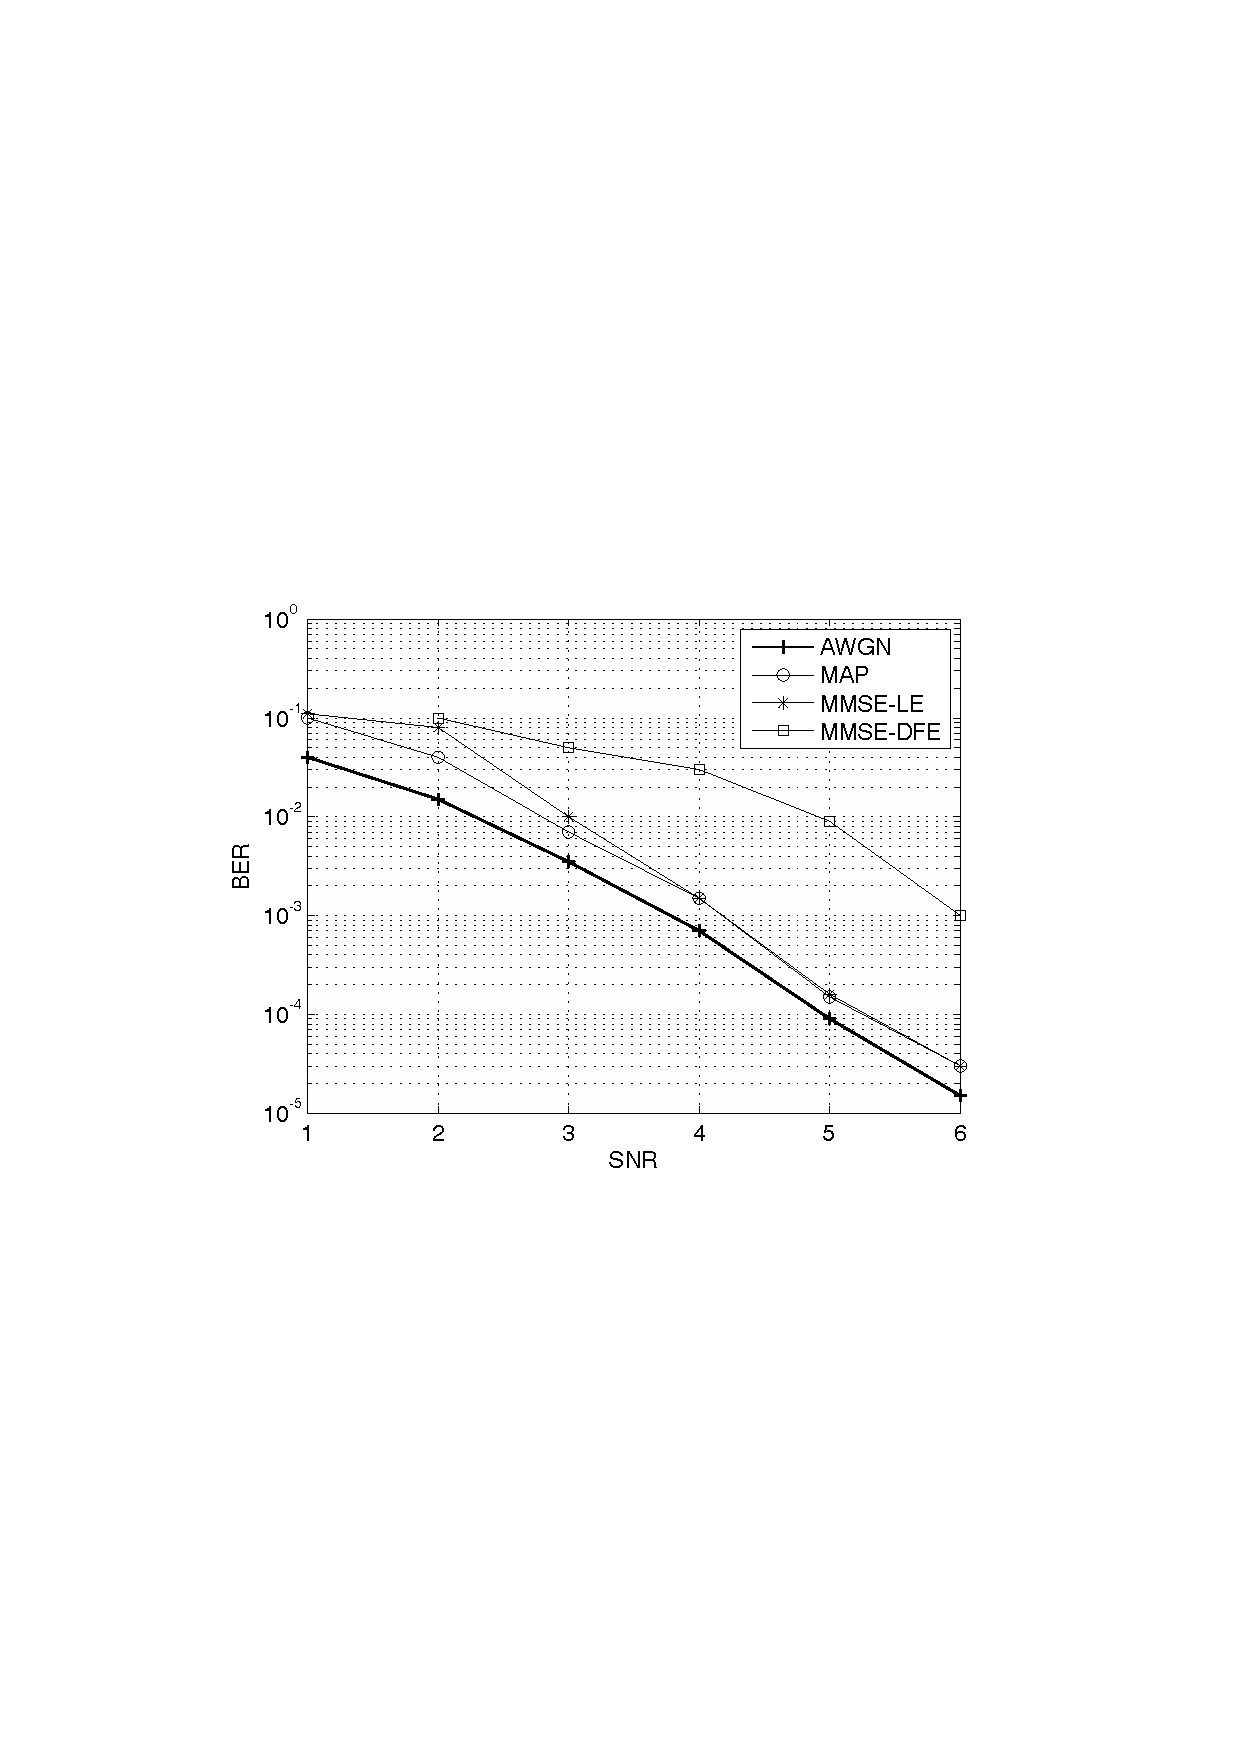
\includegraphics[width=0.8\textwidth]{images/diffcmp.pdf}
  \end{center}
  \caption{不同Turbo均衡算法的性能比较}
  \label{fig:2.5}
\end{figure}
图\ref{fig:2.5}是几种算法的性能比较,因为MAP均衡性能采用的是最优准则,在高信噪比下,经过迭代可以达到AWGN下的性能,所以性能最好,但同时复杂度也最高,不适合在实际系统中应用。MMSE-LE均衡器性能仅次于MAP均衡器,尽管传统的DFE比LE好,但是Turbo均衡应用中,基于先验信息的DFE均衡器的性能比线性MMSE均衡器差,而运算复杂度方面,二者是一样的。因此,在水声通信系统中,本文采用基于先验信息MMSE准则的线性Turbo均衡算法,并在下一章详细介绍。
%==========================================================================
\section{本章小节}
本章对海洋声学信道传输特性及其对水声通信的影响、水声信道的衰落特性及其水声多径信道模型进行了介绍和简单的分析,为水声通信系统的设计、技术参数的选取提供了重要依据。
本章介绍了LMS算法及其快速自优化算法(FOLMS)和RLS算法及其快速算法(SFTF),并给出了这两类算法的优缺点。在此基础上文献\ncite{zhaoliang}提出了一种适用于水声相干通信系统的“分集合并自最佳自适应多通道判决反馈均衡算法”,即FOLMSDC+FOLMSPC+FOLMS算法,最后并与\ncite{Stojanovic1995reduced}作比较,在性能和运算量上都有很大的优势。

另外介绍了与传统均衡算法结构不同的Turbo均衡技术,并对其中的几种均衡算法的运算复杂度以及性能加以比较,得出适用于水声通信系统的基于先验信息MMSE准则的线性Turbo均衡算法。
%%========================================================================
% empty page for two-page print
%\ifthenelse{\equal{\ioaside}{T}}{%
%  \newpage\mbox{}%
%  \thispagestyle{empty}}{}
%%========================================================================
%\end{document}
\clearpage{\pagestyle{empty}\cleardoublepage}
